\chapter{Using Business Analytics Tools for Decision Support with MATSim}
\label{ch:businessanalytics}
% ##################################################################################################################

\hfill \textbf{Authors:} Alexander Erath and Pieter Fourie

\begin{center} 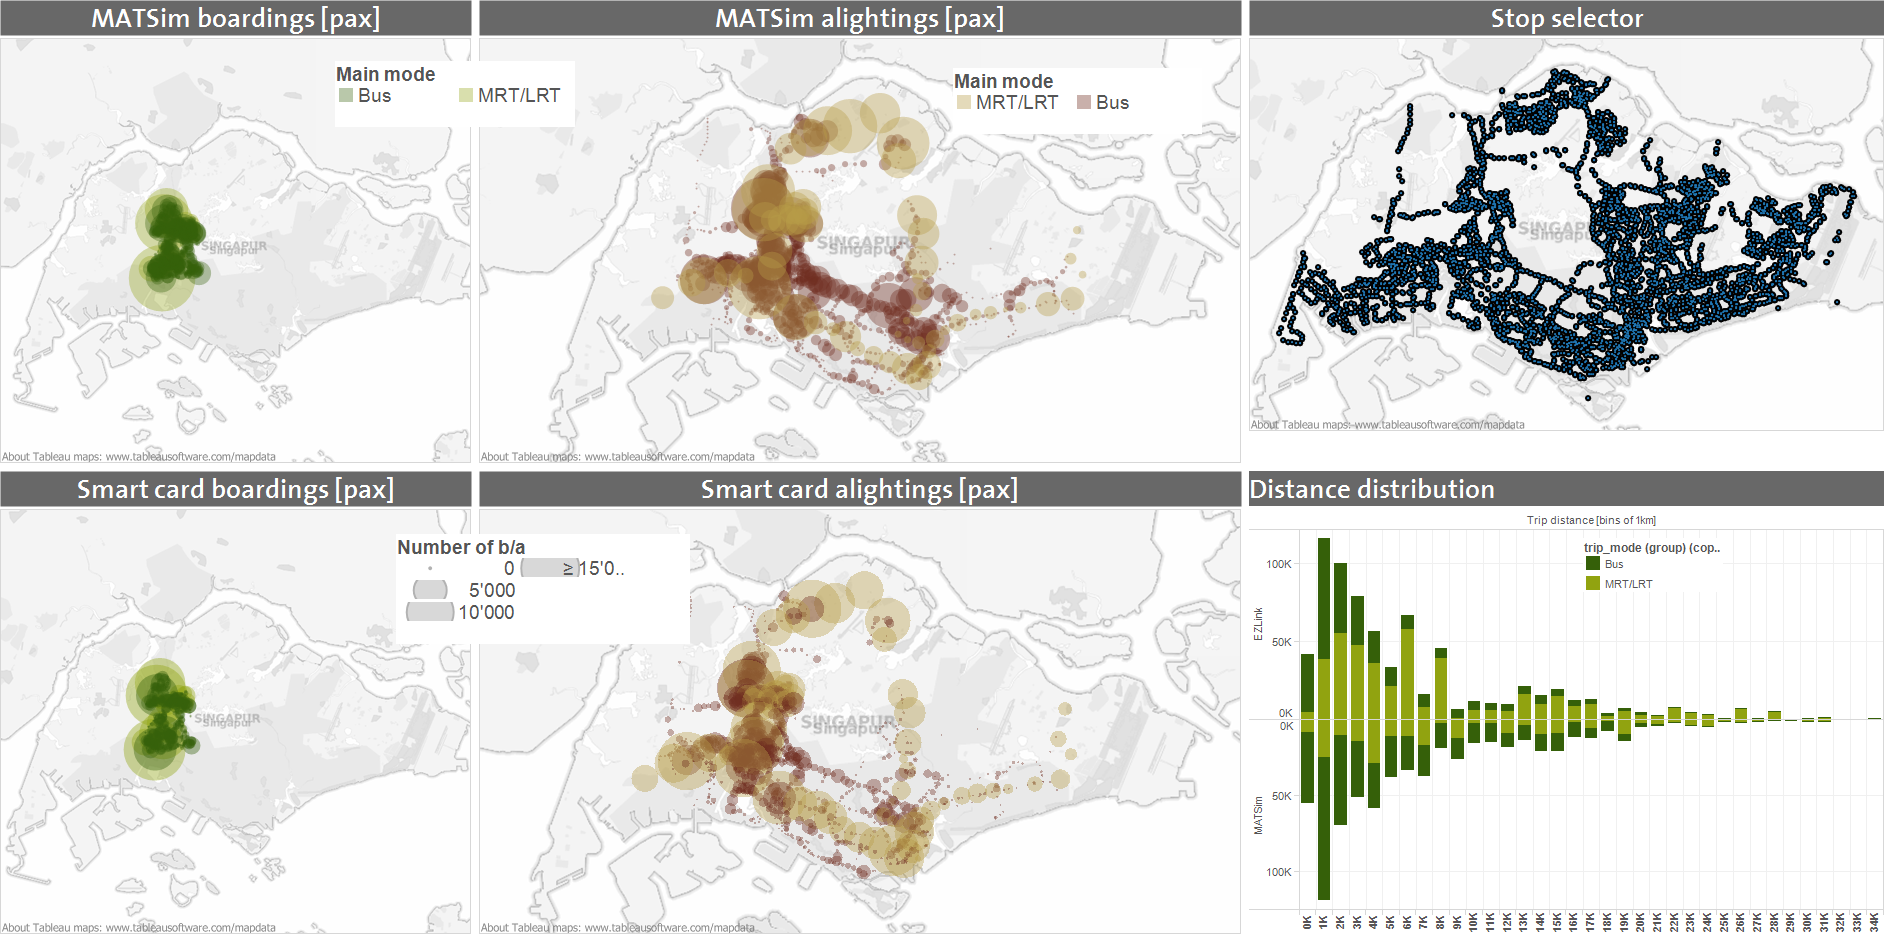
\includegraphics[width=0.4\textwidth, angle=0]{extending/figures/businessanalytics/tableau.png} \end{center}

% ##################################################################################################################

With the progress in transport demand modeling from aggregated, static and zone-based
assignment models to fully dynamic agent- and activity-based transport simulations, the scope of
data that needs to be collected, managed and maintained has changed dramatically. Furthermore,
the type of analyses as well as potential analysts have changed. Whereas traditionally transport
modelers would analyze data and create static maps, pre-defined graphs and tables we envision
other end-users: transport authorities, architects, policy-makers and the service industry. These
analysts can utilize a decision-support tool, based on the output of an agent-based model as well
as analyze their own datasets and fully analyze spatial and temporal agent behavior without
requiring continuous support from a transport modeler.

In this chapter, we present a framework of a decision support system designed to enable analysis
of the wealth of information provided by agent-based transport demand models, travel diary
surveys and automatically collected data on transport infrastructure usage \citep[see also][]{ErathEtAl_unpub_EASTS_2013, ErathEtAl_unpub_STRC_2013}. We present a practical application of the framework using it for analyzing the MATSim model of Singapore along with
the Household Interview Travel Survey and public transport smart card transaction data. At
the time of writing, the status of presented applications is only preliminary as not all necessary
dataset and interfaces are yet fully developed, but the presented case-studies give already a very
good idea about the potential scope and functioning of the decision support system. For future
work, we envisage stakeholder workshops to better understand their diverse requirements and
jointly refine what type of questions the decision support system should support to answer and
adapt it accordingly.

% ------------
\createfigure%
{Tableau visualization}%
{Tableau visualization of public transport ridership from a MATSim simulation compared against actual smart card data records in Singapore}%
{\label{fig:analyticsTableau}}%
{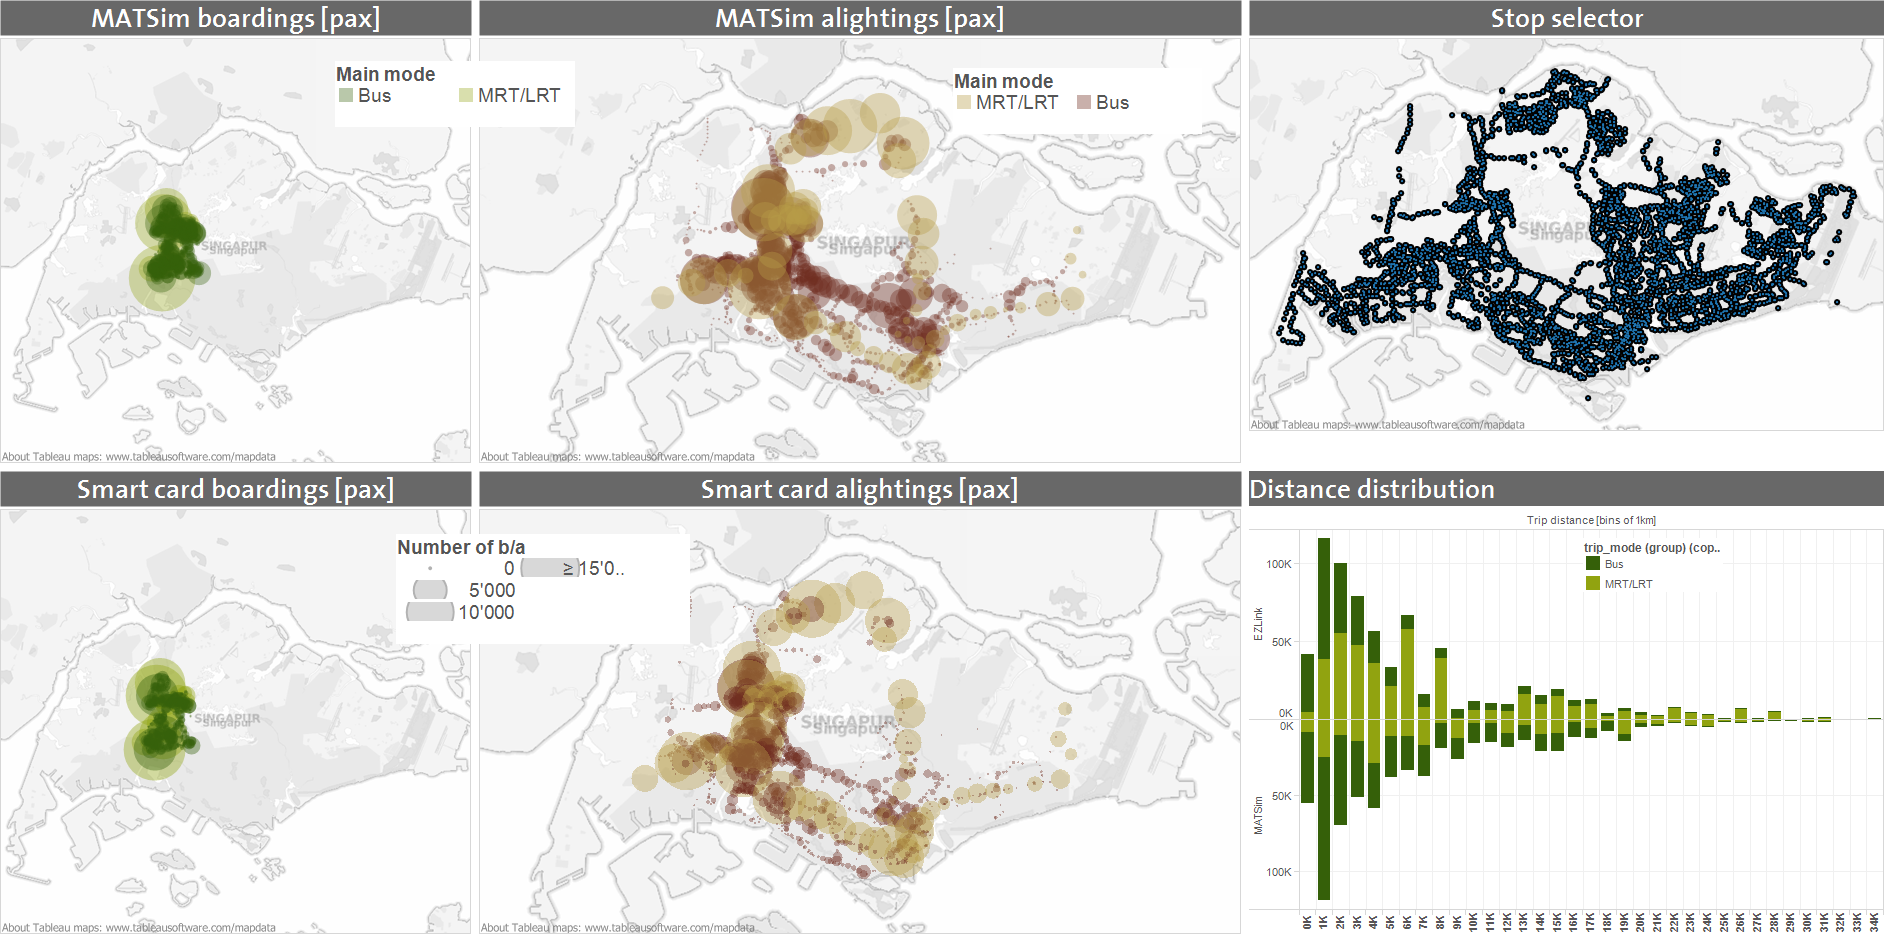
\includegraphics[width=0.25\textwidth, angle=0]{extending/figures/businessanalytics/tableau.png}}%
{}
% ------------

% ------------
\createfigure%
{General framework of the decision support system}%
{General framework of the decision support system}%
{\label{fig:analyticsFramework}}%
{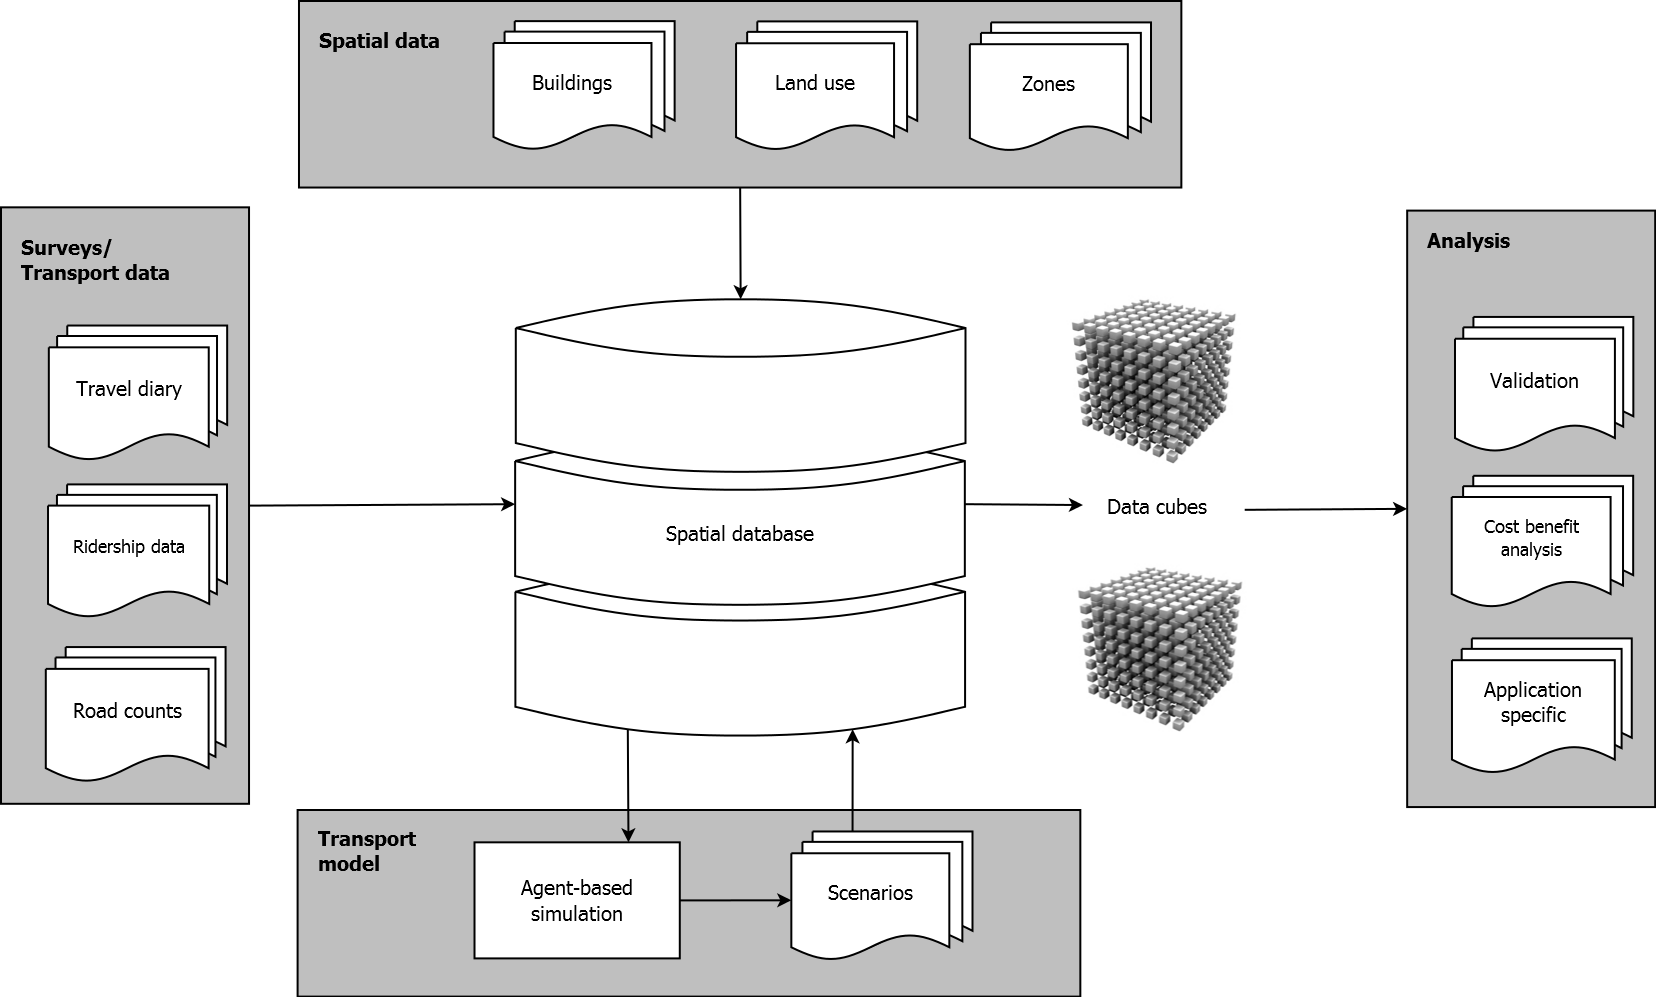
\includegraphics[width=0.65\textwidth, angle=0]{extending/figures/businessanalytics/general}}%
{}
% ------------

% ------------
\createfigure%
{Simplified entity relationship diagram showing shared keys across tables}%
{Simplified entity relationship diagram showing shared keys across tables}%
{\label{fig:analyticsERD}}%
{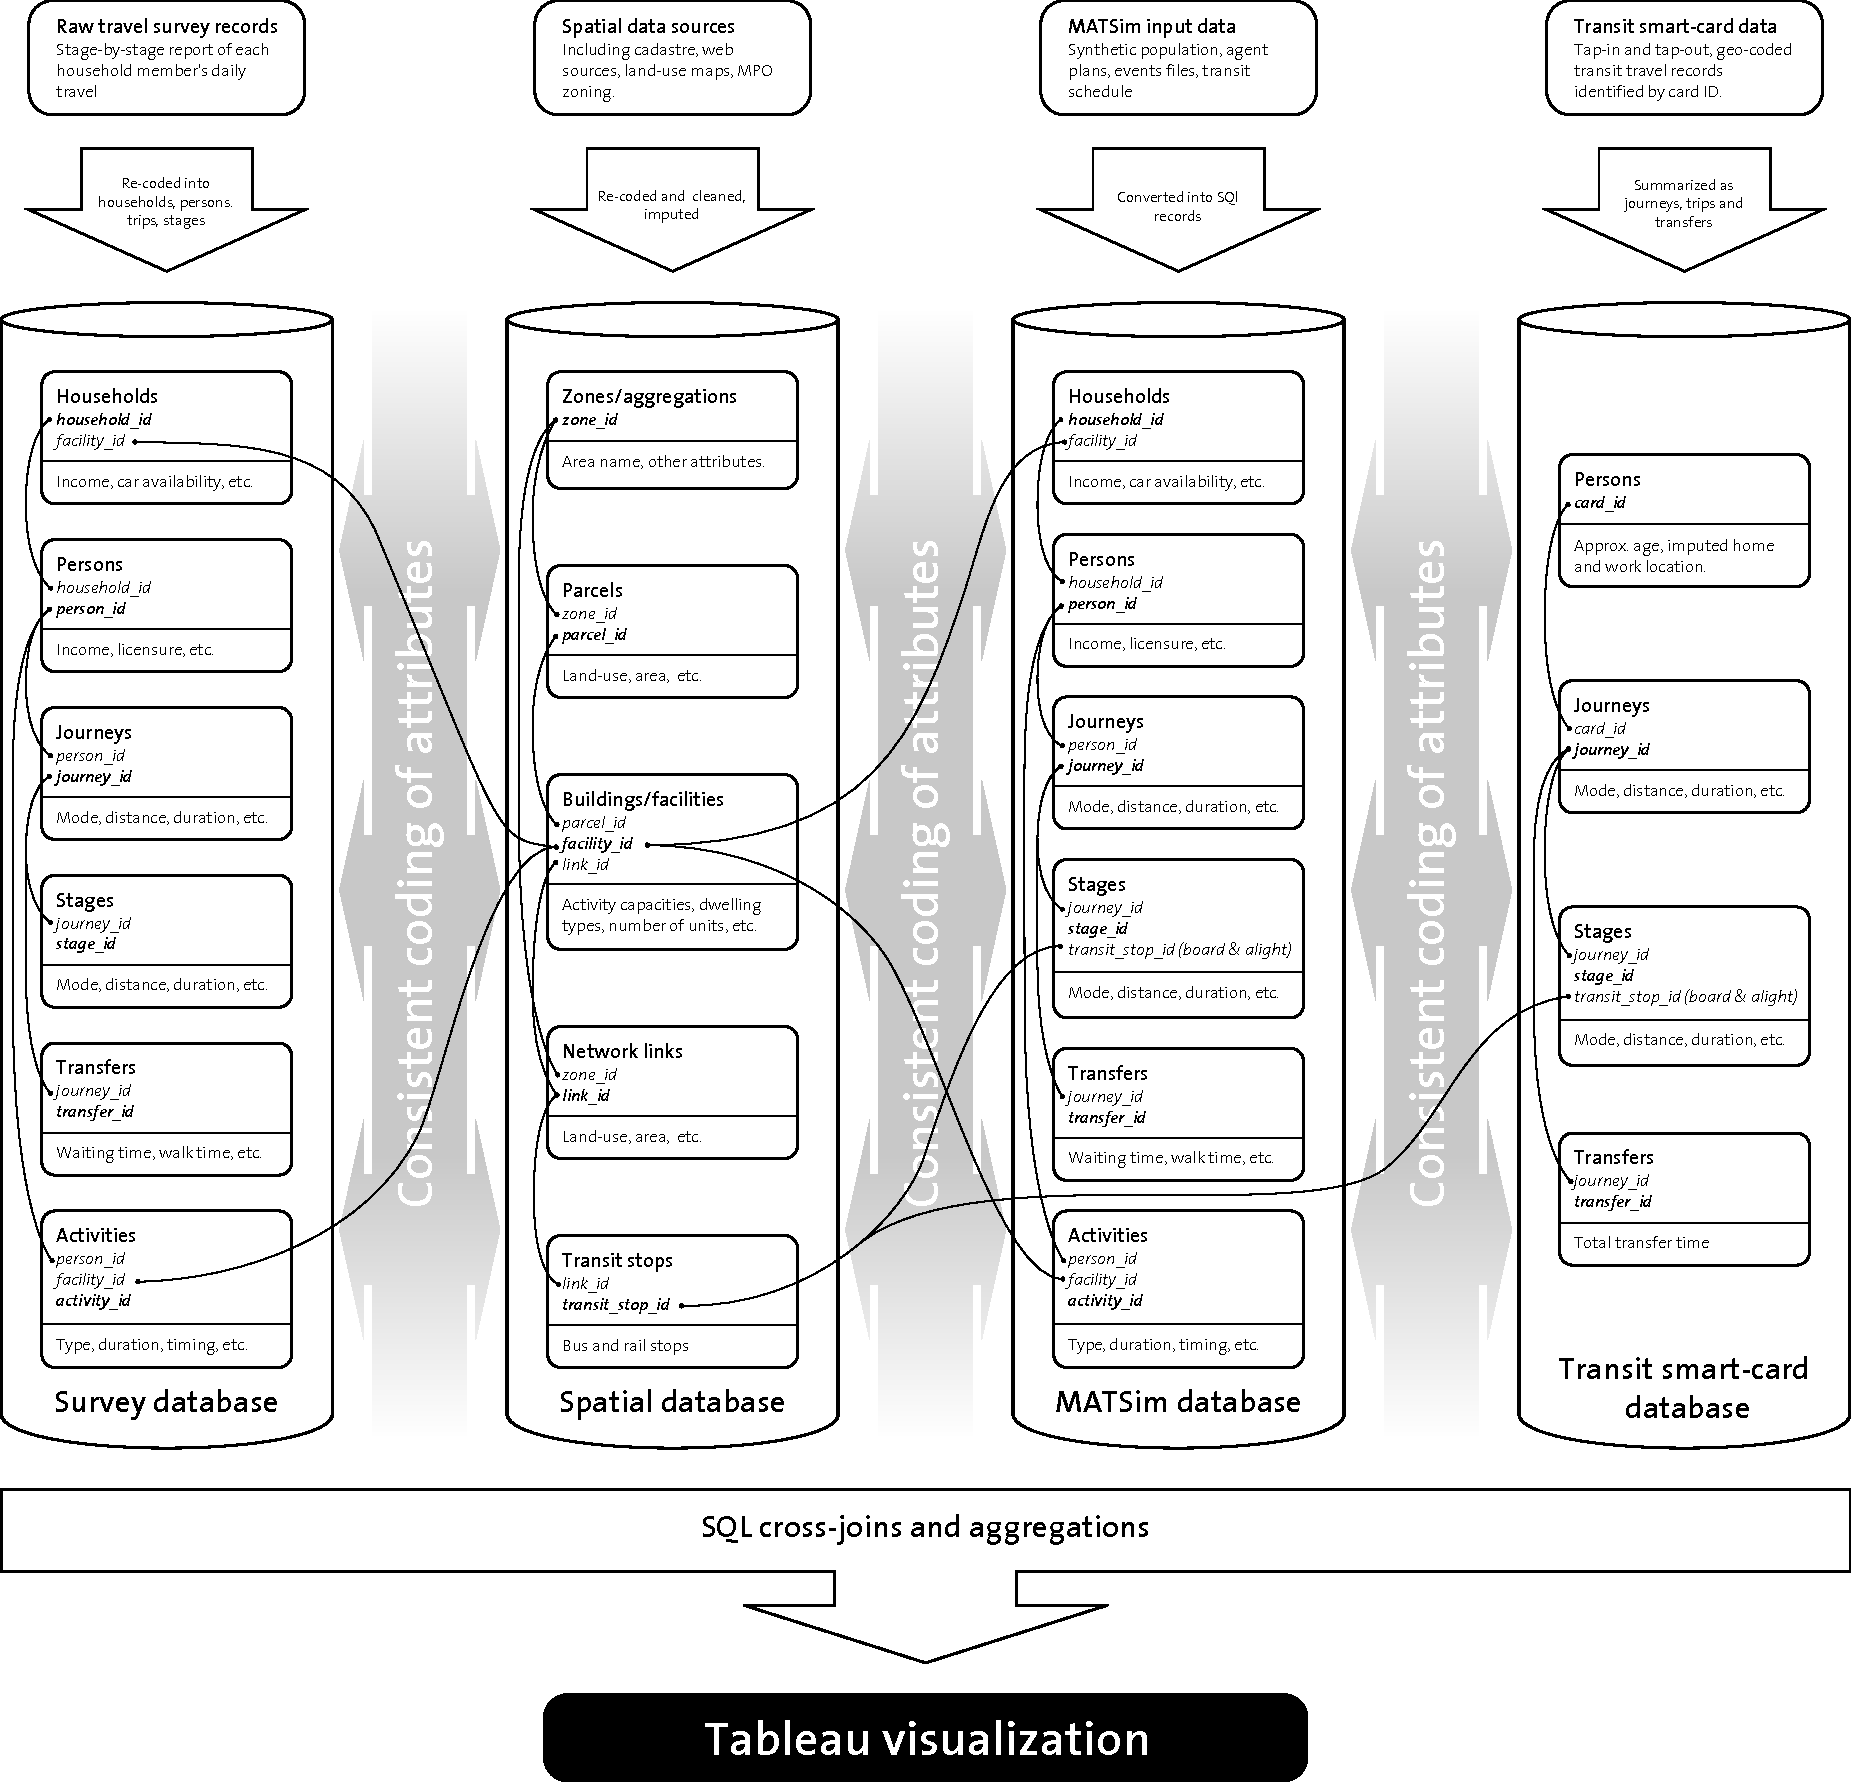
\includegraphics[width=0.65\textwidth, angle=0]{extending/figures/businessanalytics/schema}}%
{}
% ------------

% ------------
\createfigure%
{Table joined in analytics software}%
{A diagram showing how the tables from Figure \ref{fig:analyticsERD} are joined together for visualization in business analytics software, e.g. Tableau, as shown in Figure~\ref{fig:analyticsTableau}}%
{\label{fig:analyticsFramework}}%
{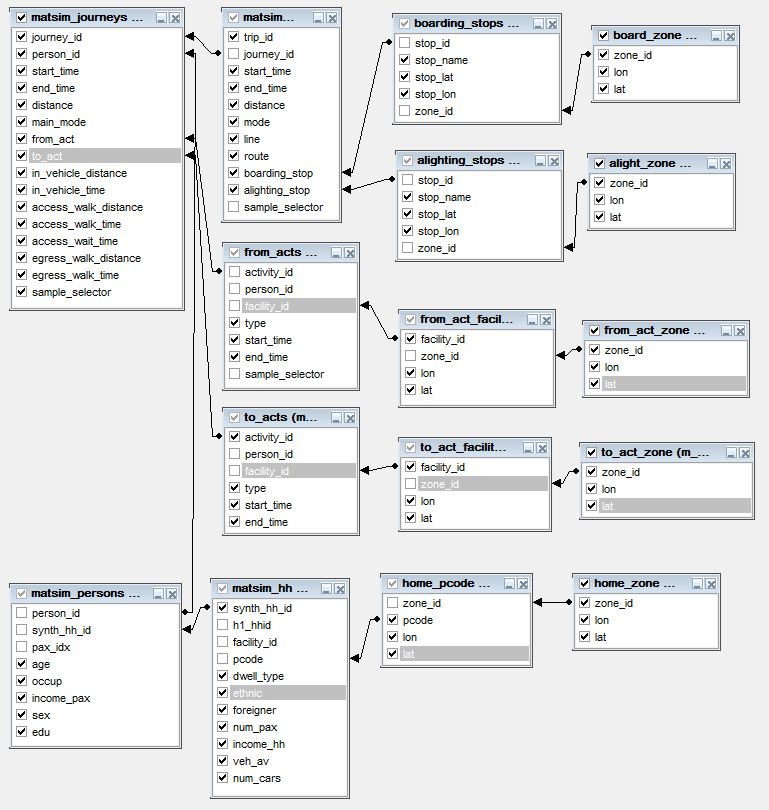
\includegraphics[width=0.65\textwidth, angle=0]{extending/figures/businessanalytics/join}}%
{}
% ------------


% ################################################################################################################
\section{Diaries from Events}
In the package \lstinline|playground.singapore.travelsummary| the reader may find a set of classes that will transform their MATSim simulation results into a set of travel diary tables, such as those discussed in the preceding section.

% ################################################################################################################




